\setcounter{page}{1}
%\section*{Zielsetzung}
%Mit dem Versuch soll das Schwingverhalten eines elektrischen Schwingkreises,
%bei Dämpfung oder äußerer Anregung, untersucht werden.

\section{Theorie}

Für einen elektrischen Schwingkreis benötigt man grundsätzlich
Kondensatoren und Spulen. %stil
Bei einer einmalig äußeren Anregung z.\,B. durch eine Peakimpuls %einmaligen, einen Nadelimpuls
kann, dann eine Schwingung gemessen werden. %kein Komma, Satz überarbeiten
Wird zusätzlich noch ein Widerstand mit angeschlossen, ergibt sich ein
gedämpfte elektrischer Schwingkreis. %gedämpfter
Wird der Schwingkreis kontinuierlich von außen angeregt, nennt man
ihn erzwungenen Schwingkreis.

\subsection{Gedämpfter Schwingkreis}
\begin{figure}
  \centering
  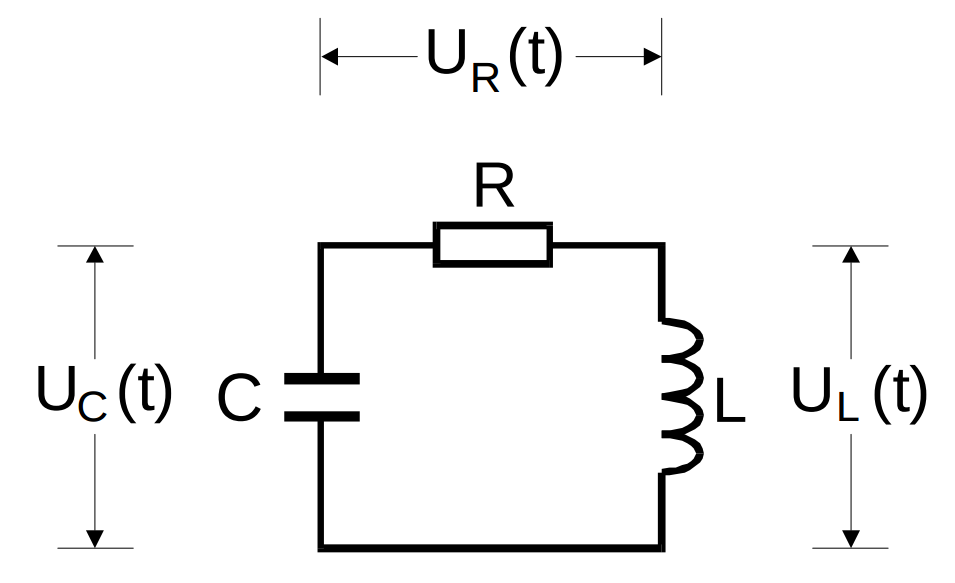
\includegraphics[width = 0.5\textwidth]{bilder/gedaempfter_schwingkreis.png}
  \caption{Schematischer Aufbau eines gedämpften Schwingkreises\cite{anleitung354}. }
  \label{fig:gedaempft}
  \end{figure}
Zunächst sollen mithilfe der zweiten %mit Hilfe
Kirchhoffschen Regel die Spannungen in einem Schwingreis (vgl. Abb \ref{fig:gedaempft}) %kreis
bestimmt werden:

\begin{equation}
  \label{eq:kirch}
U\ua{R}(t)+U\ua{C}+U\ua{L}(t).
\end{equation}

Durch hinzu nahme der bekannten Zusammenhänge %Hinzunahme

\begin{equation*}
U\ua{R}(t)=RI(t) \quad U\ua{C}(t)=\frac{Q(t)}{C} \quad U\ua{L}(t)=L\frac{\map{d}}{\map{d}t}I
\end{equation*}

und der zeitlichen Ableitung von \eqref{eq:kirch}, auf eine Schwingungsdifferentialgleichung %Verb fehlt

\begin{equation}
  \label{eq:differntialgleichung_1}
\frac{\map{d}^2}{\map{d}t^2}I+\frac{R}{L}\frac{\map{d}}{\map{d}t}I+\frac{1}{LC}I=0
\end{equation}

geschlossen werden.
Als Lösungsansatz wählt man:

\begin{equation*}
  I(t)=A\,\map{e}^{-\map{i}\hat{\omega} t} \quad A,\omega\in\mathbb{C}.
\end{equation*}
Dabei ist $\omega$ die Frequenz mit der das System schwingen kann.
Durch einsetzen von $I(t)$ in \eqref{eq:differntialgleichung_1} ergibt sich %Einsetzen
für diese:

\begin{equation}
  \label{eq:omega_gedaempft}
  \hat{\omega}_{1,2}=\map{i}\frac{R}{2L}\pm\left(\,\underbrace{\frac{1}{LC}}_{:=\omega_0}-\underbrace{\frac{R^2}{4L^2}}_{:=\beta}\,\right)^{\frac{1}{2}}.
\end{equation}

 Die Frequenz $\omega$ kann folglich drei mögliche Werte annehmen.
 Je nachdem, was für Werte $\omega_0$ und $\beta$ besitzen.  %'was' ist umgangssprachlich
\\

Bei dem Fall $\omega_0<\beta$ handelt es sich um den sogenannten \emph{Kriechfall}. %Bei dem Fall ist umgangssprachlich
 Hierbei wird die Wurzel in \eqref{eq:omega_gedaempft} negativ. Als Lösung für
 $I(t)$ erhält man

\begin{equation*}
     I(t)=A\,\map{e}^{\left(-\frac{R}{2L}\mp\sqrt{\frac{R^2}{4L^2}-\frac{1}{LC}}\right)\,t}.
\end{equation*}

Die Stromstärke besitzt somit keine periodische Eigenschaft.
\\

Ist $\omega_0>\beta$ so untersucht man den \emph{Schwingfall}. %Komma zwischen Haupt und Nebensatz
Bei diesem bleibt die Wurzel in \eqref{eq:omega_gedaempft} positiv. Als
Lösung für $I(t)$ folgt

\begin{equation*}
  I(t)=A\,\map{e}^{\left(-\frac{R}{2L}\pm\sqrt{{\frac{1}{LC}}-\frac{R^2}{4L^2}}\right)t}.
\end{equation*}

Abschließend soll der Fall $\omega_0=\beta$ besprochen werden.
Dieser wird auch als \emph{aperiodischer Grenzfall} bezeichnet.
Die Stromstärke hat hier keine Nullstellen und fällt schneller als
beim Kriechfall.
Für die Amplitude der Stromstärke ergibt sich

\begin{equation}
  \label{eq:ap_grenz}
  I(t)=A\,\map{e}^{-\frac{R}{2L}\,t}=A\,\map{e}^{-\frac{1}{\sqrt{LC}}\,t}.
\end{equation}

\subsection{Erzwungene Schwingung}
\begin{figure}
  \centering
  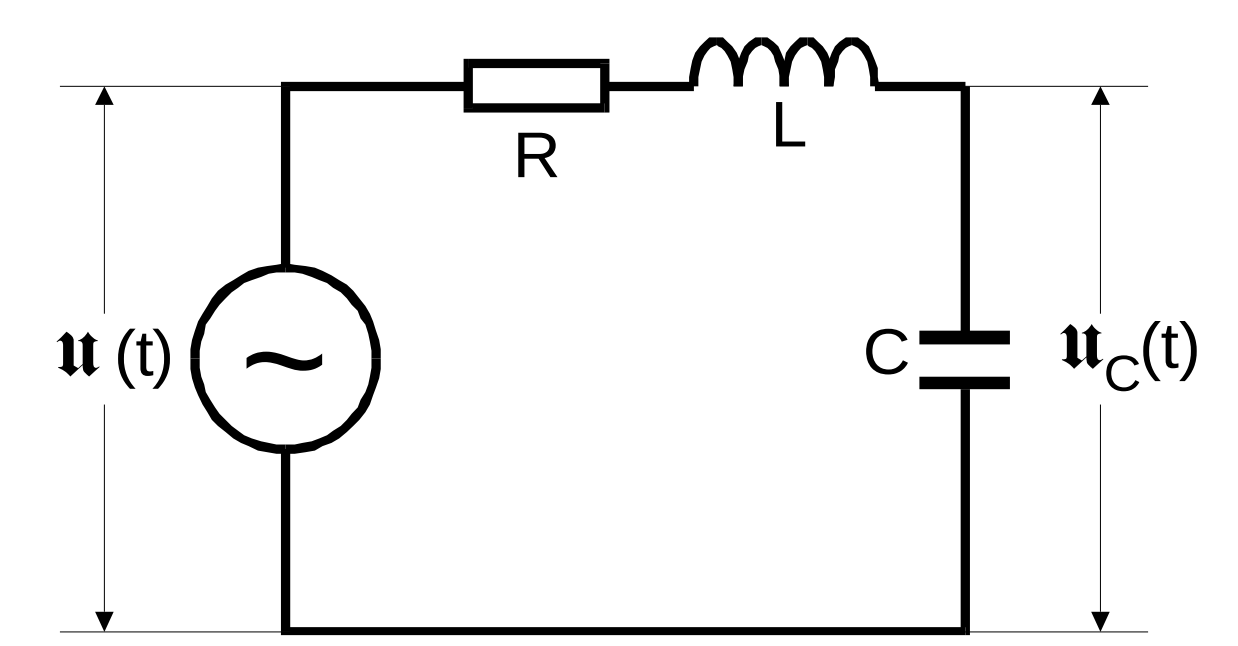
\includegraphics[width = 0.5\textwidth]{bilder/erzwungener_kreis.png}
  \caption{Schematischer Aufbau eines erzwungenen Schwingkreises\cite{anleitung354}. }
  \label{fig:erzwungen}
\end{figure}

Durch das hinzuschalten einer externen Anregung $U(t)$ (vgl. Abb. \ref{fig:erzwungen}) %Hinzuschalten
erhält die Differntialgleichung \eqref{eq:differntialgleichung_1} eine %Differentialgleichung
Inhomogenität:

\begin{align}
  \frac{\map{d}^2}{\map{d}t^2}I+\frac{R}{L}\frac{\map{d}}{\map{d}t}I+\frac{1}{LC}I=U(t)&=U_0\map{e}^{\map{i}\omega\, t}\notag \\
  LC\frac{\map{d}^2}{\map{d}t^2}U\ua{C}+\frac{R}{C}\frac{\map{d}}{\map{d}t}U\ua{C}+U\ua{C}&=U_0\map{e}^{\map{i}\omega\, t}. \label{eq:dgl_2}
\end{align}

Die Differntialgleichung \eqref{eq:dgl_2} wird gelöst durch

\begin{equation}
  \label{eq:uc_erzwung}
  U\ua{C}(\omega)=U_0\left(\left(1-LC\omega\right)1^2+\omega^2R^2C^2\right)^{-\frac{1}{2}}.
\end{equation}

Die Spannung am Kondensator ist also abhängig von der Erregerfrequenz $\omega$.
Die Untersuchung des Randverhaltens von \eqref{eq:uc_erzwung} liefert

\begin{equation*}
  \lim_{\omega \to \infty} U\ua{C}(t)=0 \qquad \lim_{\omega \to 0} U\ua{C}(t)=U_0.
\end{equation*}

Zusätzlich gibt es die sogenannte \emph{Resoanzfrequenz}.
Bei dieser Frequenz erreicht $U_C$ ihren Maximalwert. Dies ist genau dann der Fall, wenn
$\omega$ auf

\begin{equation*}
  \label{eq:resonanzfrequenz}
  \omega\ua{res}=\left(\frac{1}{LC}-\frac{R^2}{2L^2}\right)^{\frac{1}{2}}
\end{equation*}

eingestellt ist.
Die Spannungsamplitude hat folglich den Betrag:

\begin{equation}
  \label{eq:spann_ampli}
  U\ua{C,\, max}=\frac{1}{R}\sqrt{\frac{L}{C}}U_0=qU_0.
\end{equation}
Der Faktor $q$ wird auch als \emph{Güte des Schwingkreises} bezeichnet.
Ist $U\ua{C}=U\ua{C,\, max}$ spicht man von \emph{Resonanz}.
Als Indikator für die Schärfe der Resonanz dienen die beiden
Frequenzen $\omega_+$ und $\omega_-$. An diesen Frequenzen ist
$U\ua{C}$ auf

\begin{equation*}
   U\ua{C}=2^{-\frac{1}{2}} U\ua{C,\, max}
\end{equation*}

abgefallen.
Mit der Gleichung \eqref{eq:spann_ampli} und der Annahme $\frac{R^2}{L^2}\ll \frac{1}{LC}$
folgt

\begin{equation}
  \label{eq:omega_+_-}
  \omega_+-\omega_-\approx \frac{R}{L}.
\end{equation}

Die Folgerung steht durch, %kein Komma

\begin{equation*}
  q=\frac{1}{\sqrt{LC}\left(\omega_+-\omega_-\right)}
\end{equation*}

im direktem Zusammenhang mit der Güte.

Die Phasen zwischen Kondensator- und Errergerspannung kann maximal
einen Unterschied von $\pi$ besitzen. Dies folgt mit der, aus der
Herleitung von \eqref{eq:uc_erzwung} bekannten, Gleichung:

\begin{equation}
  \label{eq:phase}
  \varphi(\omega)=\arctan\left(\frac{-\omega RC}{1-LC\omega^2}\right).
\end{equation}
%Formel für Abklingzeit und R_ap
